\documentclass[tikz,border=0pt]{standalone}
\usepackage{amssymb}
\usepackage{tikz}
\usetikzlibrary{arrows.meta}

\definecolor{ink}{HTML}{0F172A}
\definecolor{muted}{HTML}{64748B}
\definecolor{gridline}{HTML}{CBD5E1}

\begin{document}
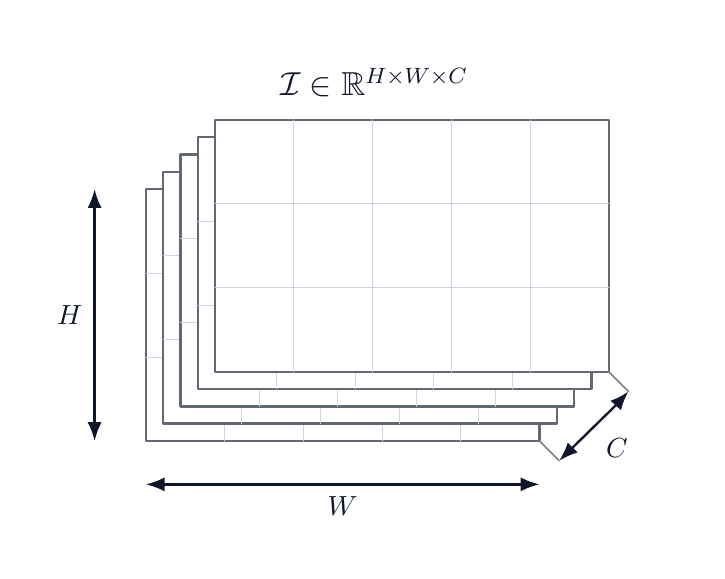
\begin{tikzpicture}[
  font=\sffamily,
  >=Latex,
  line cap=round,
  line join=round
]
  \fill[white] (-1.5,-1.4) rectangle (7.0,5.25);

  % Several two-dimensional image planes, offset to show a channel stack.
  \foreach \layer in {0,...,4} {
    \begin{scope}[xshift=\layer*0.22cm,yshift=\layer*0.22cm]
      \draw[ink!65, line width=0.9pt, fill=white] (0,0) rectangle (5,3.2);
      \foreach \column in {1,...,4} {
        \draw[gridline, line width=0.35pt]
          (\column,0) -- (\column,3.2);
      }
      \foreach \row in {1,...,2} {
        \draw[gridline, line width=0.35pt]
          (0,\row*1.0667) -- (5,\row*1.0667);
      }
    \end{scope}
  }

  \draw[ink, <->, line width=0.85pt]
    (-0.65,0) -- (-0.65,3.2)
    node[midway, left=3pt, fill=white, inner sep=1pt] {$H$};
  \draw[ink, <->, line width=0.85pt]
    (0,-0.55) -- (5,-0.55)
    node[midway, below=3pt, fill=white, inner sep=1pt] {$W$};
  % Channel depth: measure the offset from the back sheet to the front sheet.
  \draw[ink!55, line width=0.55pt] (5,0) -- (5.25,-0.25);
  \draw[ink!55, line width=0.55pt] (5.88,0.88) -- (6.13,0.63);
  \draw[ink, <->, line width=0.85pt]
    (5.25,-0.25) -- (6.13,0.63)
    node[midway, below right=3pt, fill=white, inner sep=1pt] {$C$};

  \node[ink, font=\large] at (2.9,4.55)
    {$\mathcal{I} \in \mathbb{R}^{H\times W\times C}$};
\end{tikzpicture}
\end{document}
